%
% 2010.01.24 情報システム工学科対応
% 2018.01.05 電子・情報工学科対応
%
\documentclass[10pt]{tpu-abst}
\usepackage[dvipdfmx]{graphicx}
\usepackage{listings,jlisting}
\lstset{language=C,%
    basicstyle={\ttfamily\small}, %書体の指定
    frame= tRBl, %フレームの指定
    framesep=10pt, %フレームと中身(コード)の間隔
    breaklines=ture, %行が長くなった場合の改行
    linewidth=8cm, %フレームの横幅
    lineskip=-0.5ex, %行間の調整
    tabsize=2 %Tabを何文字幅にするかの指定
	}%
%
% ここでタイトルの設定をします
%
% 自分の名前
\author{尾崎 裕樹}
%
% 学籍番号
\gakuban{1515015}
%
% 研究室の番号
\kouzanum{2}
% 1 情報基盤工学講座 
% 2 情報システム工学講座 
% 3 集積機能デバイス工学講座 
% 4 電子通信システム工学講座 
%
%
% 指導教員名: 
% \kouzaname{ななし} % これはコメントアウトする
% \kouzaname{太田} % 
% \kouzaname{奥原} % 
% \kouzaname{西田} % 
% \kouzaname{榊原} % 
\kouzaname{中村(正)} % 
% \kouzaname{松本(三)} % 
% \kouzaname{唐山} % 
% \kouzaname{鳥山} % 
% \kouzaname{岩本} % 
% \kouzaname{安宅} % 
% \kouzaname{中田} % 
% \kouzaname{浦島} % 
% \kouzaname{松田(敏)} % 
% \kouzaname{岩田} % 
% \kouzaname{松田(弘)} % 
% \kouzaname{石坂} % 
% \kouzaname{三宅} % 
% \kouzaname{小林(香)} % 
% \kouzaname{小島} % 
%
% 発表番号
\happyou{17}
%
% タイトル
\title{プログラミング演習における模範解答を\\用いたテストケース評価基準の自動生成}
%
%----- begin document
%
\begin{document}
%
\maketitle
%
%----- your abstract, please
%

\section{ はじめに}
%
プログラミング演習において,学生自身がテストケースを設計しテストを行うことによって,学生が作成したプログラムを自身で評価することができる。プログラムの正確な評価には適切なテストケースが必要なので,設計したテストケースの評価方法を考える必要がある。

そこで,テストケースが適切であるかを判定する評価基準を用意して,評価基準に対する設計したテストケースの網羅率を求めることでテストケースを評価する手法が提案されている~\cite{a1}。

本研究では,評価基準作成時における教員の負担を減らすために,テストケースの評価基準を自動化を行うことを目的とする。プログラムテストとテストケース評価基準,本研究で行う評価基準自動生成の関係を図\ref{cap1}に示す。
\begin{figure}[h]
  \centering
  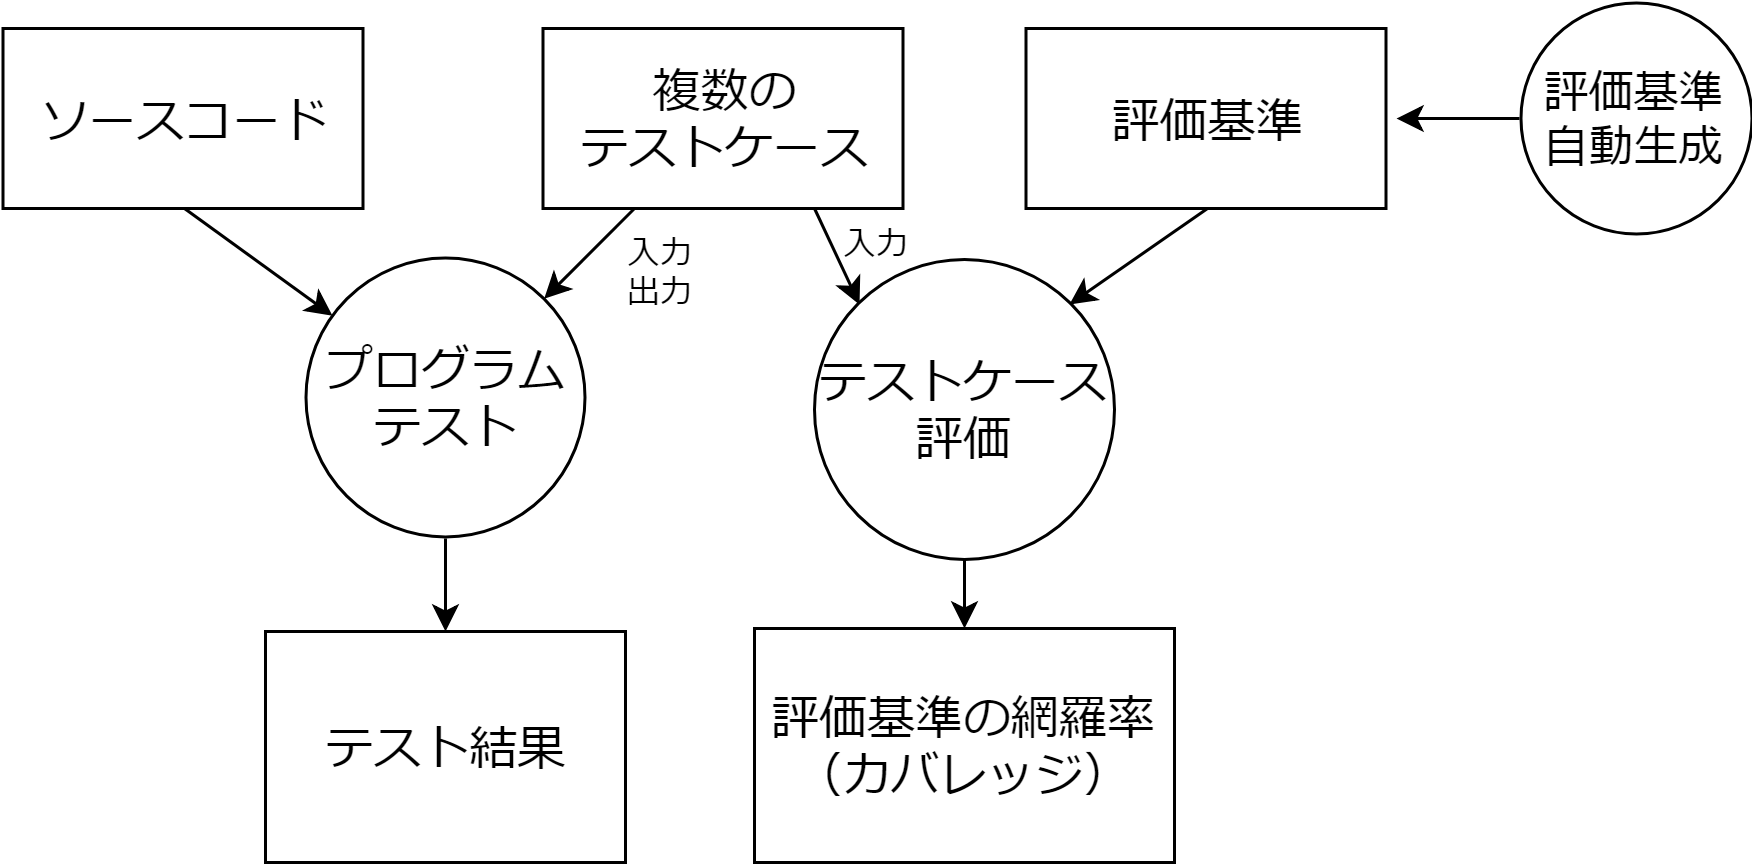
\includegraphics[width=80mm]{開発するシステムの位置づけmini3.png}
  \caption{開発するシステムの位置づけ}
  \label{cap1}
\end{figure}
%
\section{関連研究}
%
文献~\cite{a1}のテストケース評価システムでは,学生自身が適切なテストケースを設計できるようになるために,学生が作成したテストケースを評価してアドバイスを行うシステムが提案されている。このシステムでは,教員が演習問題毎にテストケースの評価基準とテストケースが不足していた場合に表示するアドバイスを与える必要がある。演習問題毎にテストしなければならない値や入力のデータ数が異なるため,評価基準は演習問題を分析した上で,入力のデータ構造を定義してから記述される。
%
\section{テストケース評価基準の自動生成}
テストケース評価システムでは,教員が問題文を分析した上で,評価基準を記述しているので,システムを運用する上で教員の負担が大きくなってしまうことが考えられる。そこで,本研究は教員の負担を減らすために,評価基準と入力のデータ構造を自動で生成する方法を提案する。

テストケース評価基準を生成する際に,問題文を分析して記述するのではなく,模範解答のプログラムを解析し,入力がある変数と条件式を抽出することによって,評価基準を生成する。
% section 3 ----
\section{プログラミング課題への適用}
参考書~\cite{b1}の練習問題を用いて作成したシステムによって評価基準が生成できているかを検証した。

入力データの型に基づく評価基準や,条件文に基づく評価基準,関数を含むプログラムに対する評価基準の生成は確認することができた。しかし,配列や繰り返し分を含むプログラムからは評価基準が生成できなかった。入力された身長と体重からbmiを計算して肥満度を表示するプログラムの条件文の一部とそこから生成される評価基準を以下に示す。
\begin{lstlisting}
条件文の一部
	if (bmi >= 25)	{
		printf("あなたは肥満です。\n");
	}else if (bmi < 18.5)	{
		printf("あなたは低体重です。\n");
	}else	{
		printf("あなたは普通体重です。\n");
	}

条件文から生成された評価基準
height <= 0 || weight <= 0
!(height <= 0 || weight <= 0)
bmi >= 25
!(bmi >= 25)
bmi < 18.5
!(bmi < 18.5)
\end{lstlisting}

% section 4 ----
\section{おわりに}
本研究では,学生が自身でテストケースの評価を行うために用いるテストケース評価基準を自動生成する方法を提案した。参考書の練習問題によって配列や繰り返し文があると評価基準が生成できないことが確認できた。

今後は,現在対応できていない配列や繰り返し文を含むプログラムからの評価基準の自動生成や,生成した評価基準を入力としてテストケースの評価が可能なシステムの作成が課題となる。

\begin{thebibliography}{2}
 \bibitem{a1} {\small 蜂巣吉成,小林悟,吉田敦,阿草清磁: プログラミング演習におけるテストケース評価システム,コンピュータソフトウェア第34巻第4号,2017,pp.54-60}
 \bibitem{b1} 高橋麻奈: やさしいC,SB クリエイティブ,2012
\end{thebibliography}
%
\end{document}